\documentclass[a4paper,10pt]{scrartcl}
\usepackage[utf8]{inputenc}

\usepackage{graphicx}
\usepackage[utf8]{inputenc} %-- pour utiliser des accents en français, ou autres
\usepackage{amsmath,amssymb,amsthm} 
% \usepackage[round]{natbib}
\usepackage{url}
\usepackage{xspace}
\usepackage[left=20mm,top=10mm]{geometry}
\usepackage{algorithmic}
\usepackage{subcaption}
\usepackage{mathpazo}
\usepackage{booktabs}
\usepackage{hyperref}
% \usepackage{hyperref}
\usepackage[utf8]{inputenc}
\usepackage{graphicx}
\usepackage{amsmath}
\usepackage{multicol}
\usepackage{amssymb}
\usepackage{listings}
\usepackage[toc,page]{appendix}
\usepackage{geometry}
\usepackage{minted}
\usepackage{todonotes}
\usepackage{svg}

\usepackage[%
    style=ieee, %apa of ieee?
    isbn=false,
    url=false,
    doi=true
]{biblatex}
\addbibresource{references.bib}

% \title{Digital Twin Based Authentication Scheme To Secure Communication With IoT Application}
\title{Digital Twin and Securing IoT Applications}

\author{Teklit Haphtu Gebremaraim \\ \url{t.h.gebremariam@student.utwente.nl}}
\date{November 2022}

\begin{document}

\maketitle

\section{Introduction}
The emergence of Digital Twins(DT) and the Internet of Things(IoT) has opened up a new opportunity for businesses to leverage technology to gain insights and optimize performance. To maintain the security and privacy of data, these technologies comes, however, with their own unique set of security challenges that must be addressed. In this paper, we will explore the current state of security, particularly the authentication scheme used to ensure the confidentiality and integrity of data flow between the virtual model, which is the DT, and the physical devices, which could be sensors or actuators. We will also provide lightweight DT based authentication scheme along with how to implement for IoT application. Finally, we will conclude our work with a recommendation on how to protect a DT and IoT network with efficient and performant cryptographic authentication schemes. 

% ----- Archive
% Over the years data has become crucial part for proper functioning of  business process. Due to the growing adoption of IoT in daily life, it is being created on a massive scale. Maintaining the confidentiality and integrity of data that is sent across communication channels is critical for the security and safety of any system. Recent years have seen an increase in interest among researchers in applying Digital Twin (DT) to challenges in a range of disciplines, including cyber security . DT are simulations of real-world physical systems and operations

\section{Motivation}

The main driving force that set us to do this study is an unresolved issue we identified in DT and IoT's digital communication.
Plus, there is also a growing desire in various business sector to transform traditional processing and automation method into efficient and optimized process via DT and IoT \cite{atalay_digital_2022}. Securing a communication channel that used for transiting sensitive data is a pressing issue that needs to be studied and improved. 



% \section{Problem Statement}
% Version one 
% Traditional security measures are no longer effective due to the low power nature of many IoT sensor nodes\cite{williams_survey_2022}, and problems like communications taking place without sufficient encryption or authentication are being reported in the literature. The large-scale data collecting that is made possible by these devices is another frightening problem. If proper security measures (authentication, authorization, encryption, and so on) are not used, an attacker may be able to perform a man in the middle attack with the intent of intercepting sensitive sensor data or disrupting a system by injecting his own fault data\cite{nguyen_survey_2021}.
% The innovative idea of Digital Twins (DTs) has been adopted by research and industry more frequently since 2017 in a variety of disciplines, including industrial production, the process industry, building management, the health care sector, and smart cities. 


% Version 2
Manufacturing facilities, including critical infrastructure,  are using IoT sensors to collect and send sensor measurement and operating conditions to Digital Twin station to monitor and optimize the overall operation of the business process \.  However, due to storage and processing constraint IoT sensors have[ \cite{williams_survey_2022}, \cite{noauthor_lightweight_nodate}], it is challenging to adopt traditional security cryptographic mechanisms and ensure the confidentiality and integrity of data flow between IoT and DT. If proper security measures (authentication, authorization, encryption, and so on) are not used, an attacker may be able to perform a man-in-the-middle attack with the intent of intercepting sensitive sensor data or disrupting a system by injecting his crafted faulty data. In previous literatures and standard bodys, it is mentioned to utilize security schemes that can fit into constraint devices to address the security requirement. Hence, in this paper, we propose a lightweight mutual authentication scheme to ensure the security of IoT applications in Digital Twin.


\section{Research Question}
In this paper, we are attempting to answer the following research questions: 
\begin{itemize}

    % RQ 1
    % \item RQ1. What mututal authentication schemes for DT and IoT application are discussed in the literature? 
    % \item How can we use Digital Twin to enhance security issue in IoT/IIoT application? 
    %  Replace schemes by  mechansims.
    \item \textbf{RQ1}: What are the security schemes presented in the literature to ensure the authentication between Digital Twin and its mapped physical devices? 
    This research question will be answered through systematic literature review with the following subcategory research questions.
    \begin{itemize}
        \item{ \textbf{RQ1.1}: What is the concrete concept of Digital Twin}
        \item{ \textbf{RQ1.2}: How Digital Twin is used to enhance the security of IoT applications}
    \end{itemize}

    % RQ 3
    % 
    \item \textbf{RQ2}: How to ensure the security requirement of digital communication between a Digital Twin and companion physical IoT device. 
    
    % Research Question 4
    % \item What are the performance and efficiency differences between the proposed scheme and the existing solutions presented in the literature?
    \item \textbf{RQ3}: What is the performance analysis comparison of using proposed scheme and the existing solution presented(discussed) in the literature? 
    % update the above question 
\end{itemize}

% \section{Background}

\section{Research Methodology}

\subsection{SLR Methodology Planning Protocol}
% 3 section our plan to answer the four mentioned questions 
In order to address the first research question(\textbf{RQ1}), a systematic literature review will be carried out in this paper. During the systematic literature review the main theme is to identify the security schemes presented in the literature to ensure the authentication of data flow between the virtual world(DT) and the physical object(sensors). Under subcategory of this main question, the concept of Digital Twin will be also studied and analysed. In this section, we briefly describe the planning protocol methodology for conducting systematic literature review as follow. 

Based on the first research question(\textbf{RQ1}), we identify 5 key terms that we plan to use for retrieving research articles from research databases, these are "Digital Twin", "IoT" "Authentication", "Security", and "communication". The first three key terms are most important keywords and SHOULD be included together in the paper. where as, the last two key terms are not mandatory to be present in the paper. The main key terms and their accepted variants are outline in Table \ref{keyterms}. 

\begin{table}[!ht]
    \centering
    \begin{tabular}{|l|l|}
    \hline
        \textbf{Key terms} & \textbf{Varients / Synonyms / Similar Semantic Meaning} \\ \hline
        Digital Twin & DT, Digital-Twin, Digital-Twins, Twins, Digitalization, Virtual Clone \\ \hline
        Internet of Things & IoT, Sensors, Actuators,  \\ \hline
        Authentication & Certificate, Verification\\ \hline
        Security & Integrity, Confidentiality, Cybersecurity,  \\ \hline
        Communication & Channel, message, messages \\ \hline
    \end{tabular}
    \caption{Main Keyterms }
    \label{keyterms}
\end{table}

As a base for searching relevant literature we use of well know computer science archives: IEEE Xplore according to \cite{kofod-petersen_how_nodate} and Scopus. In this systematic literature review part of the project, we only focus on articles published between 20016 and 2022 (7 years). The reason we choose those date is, according to systematic literature conducted by Kukushkin et al. \cite{kukushkin_digital_2022}, majority Digital Twin related articles are published in the last seven years.
\\
The following table shows few offline and online tools we used in for the systematic literature review. 
\begin{table}[!ht]
    \centering
    \begin{tabular}{|l|l|}
    \hline
        \textbf{Name of Tools} & \textbf{Purse / Function} \\ \hline
        Excel & To remove duplication, get insight \\ \hline
        VOSviewer & Bibliometric analysis \\ \hline
        Researchrabbit & For validating VOSviewer map,  \\ \hline
        Connectedpapers & For validating VOSviewer map,  \\ \hline
        parsifal & To document the whole systematic literature review process \\ \hline
    \end{tabular}
    \caption{Tools used for SLR  }
    \label{slrtools}
\end{table}

\subsection{Implementation Methodology}
To address research question three(\textbf{RQ3)}, we will implement our proposed authentication scheme on an open-source Digital Twin platform called Ditto and on one of microcontroller manufactured by Pycom called ESP32. The authentication scheme is based on a lightweight cryptographic algorithm standardized by NIST on March 2021.Ditto is an open source framework developed and maintained by Eclipse Foundation to facilitate the interaction between Digital Twin and IoT devices\cite{noauthor_eclipse_nodate}. We opt to ESP32 chipset because it can be programmed with micropython which is an implementation of Python3 for microcontroller. 
To answer our last research question, we will test our implementation using a power measuring tool to estimate the performance of the proposed schemes in terms of power consumption, execution time, and storage complexity.

% \begin{figure}[H]
%     \centering
%     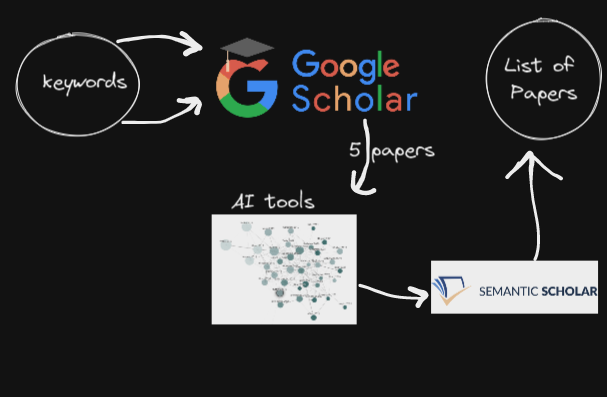
\includegraphics[width=1\textwidth]{images/method.png}
%     \caption{Research Methodology}
%     \label{fig:method}
% \end{figure}

% \subsection{Literature review methodology}
% Focus area of literatur review 
% Database used for paper extraction 
% Search keyword used
% Fiiltering mechanism 
% The tools we use to select papers. parameters used as factor of selection 

% \subsection{Problem solution methodology}

\section{Proposed Solution}
% Version 1
% Implement efficient and lightweight cryptographic authentication schemes to enhance the security of communication channel between the Digital Twin and its counterpart physical components that cloud be any IoT device.In this project we envision a light weight cryptographic scheme that can able to provide data protection at transit as well as secure access to remote IoT devices deployed on remote industry area. 

% Version 2
The IoT devices are low power and resource constraints that are not capable of running traditional cryptographic schemes like AES and RSA. Nevertheless, these devices are being widely used in various sectors including manufacturing, transportation, health, power grid, and so on, for various application. In addition, IoT sensors have also become an integral part of Digital Twin technology to collect and send data over network. In this paper, we propose an efficient and lightweight cryptographic authentication schemes to enhance the security of the communication channel between the Digital Twin and its counterpart physical components which is in most cases resource constraint IoT devices. Besides, we envision our mutual lightweight authentication scheme can also provide secure access to remote IoT device(sensors) and  Digital Twin station.

% \section{Workflow and Tools}

\begin{figure}[H]
    \centering
    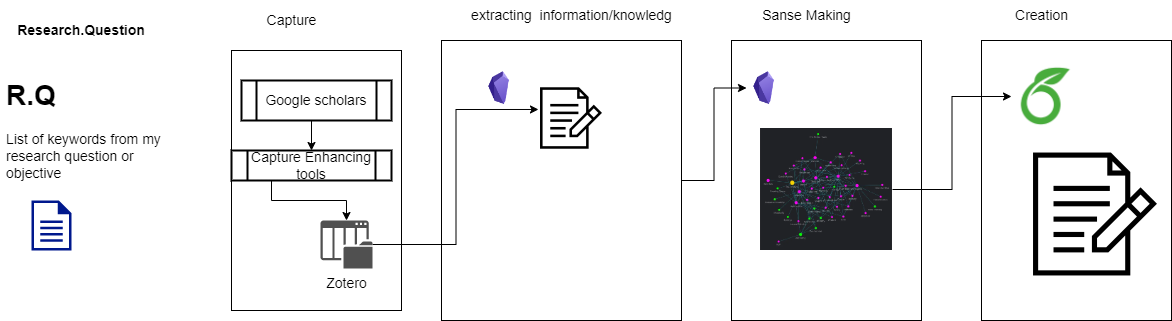
\includegraphics[width=0.8\textwidth]{images/Untitled Diagram.drawio.png}
    \caption{My workflow for my research}
    \label{fig:test_results}
\end{figure}

\section{Time Planning}

\begin{figure}[H]
    \centering
    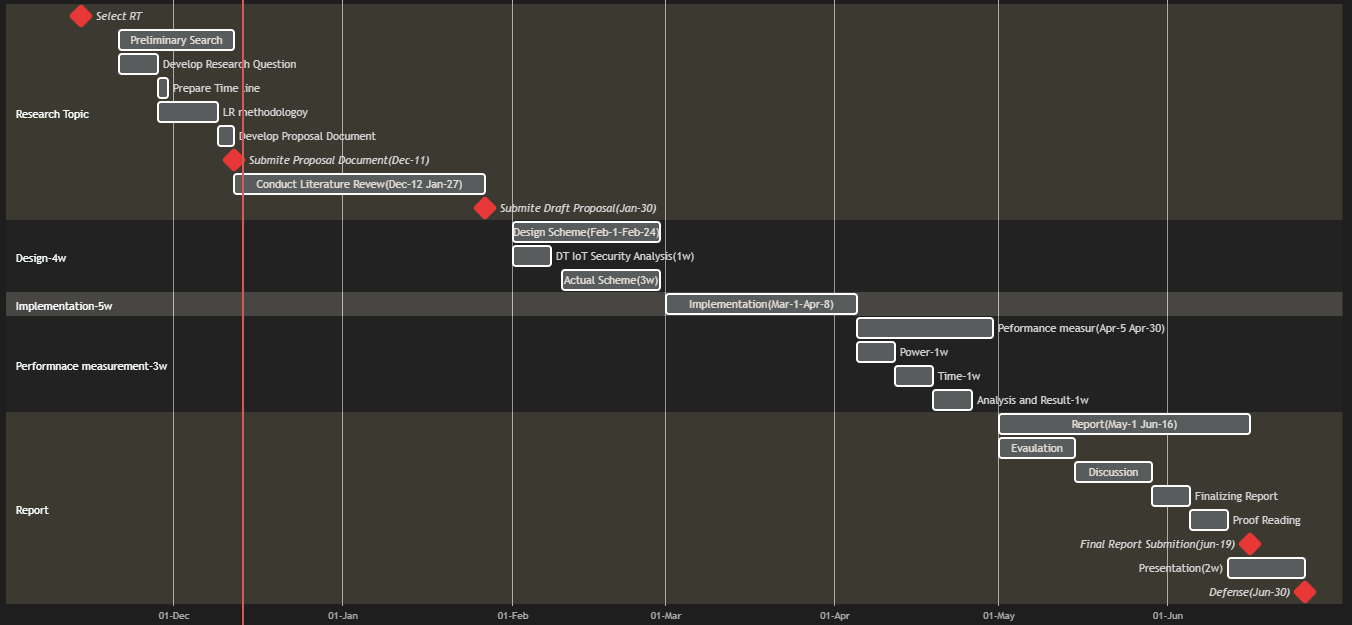
\includegraphics[width=1\textwidth]{images/plan.png}
    \caption{Research Time Plan}
    \label{fig:test_results}
\end{figure}


% \newpage
\printbibliography
\vspace{12pt}
% 12. Include references and word count


\end{document}
